\chapter{Research, Framework}\label{research-framework}

This chapter will introduce the research done prior to the design. It
will explain the motivation behind working on software development
environments, give a short history of \glspl{ide} and list typical
\gls{ui} design patterns in \glspl{ide}. It will close by presenting a
survey and a series of interviews done in order to understand the
problem space.

\section{History and role of IDEs}\label{history-and-role-of-ides}

Software development environments have been predecessed by general text
editors, starting with several projects at the Xerox \gls{parc}. Douglas
Engelbart created the text editor for the NLS system (oNLine System)
which allowed \gls{wysiwyg} style editing \cite[pp.]{moggridge}. In the
\emph{Gypsy} text editor, Larry Tesler first integrated modeless moving
of text, which is known as \emph{Copy\&Paste} \cite[pp.]{moggridge}.
Text editors with those functionalities are now the core of any software
development environment.

Later, while working with Alan Kay, Tesler created the first class
browser for the Smalltalk programming language. Class Browsers are used
to look at source code not as textual files, but as logical entities of
a programming language (for example, classes and methods). The Smalltalk
class browser was therefore the first software specifically written for
creating software, and a predecessor to any modern \gls{ide}.

\glspl{ide} integrate text editors (due to their specific purpose also
referred to as \emph{code editors}) with other software development
tools. Typically, those tools may include compiler, build system, syntax
highlighting, autocompletion, debugger, and symbol browser.

Nowadays, IDEs make use of many more \gls{ui} patterns and adapt them to
a specific purpose. Taking the Eclipse IDE as an example, one can see
that the class browser is built using a Tree View (as often seen in file
browsers), and the text editor uses bold, italic and coloured text
automatically to distinguish different entities of the programming
language (so-called \emph{syntax highlighting}).

\textbf{TODO: screenshot of eclipse w/ class browser + syntax
highlighting}

The IDE landscape is today more differentiated than ever, ranging from
minimal, purpose-specific environments like Processing to huge,
general-purpose, commercial environments like Visual Studio. Those
different IDEs serve the needs of different developers and development
situations. But still, it seems like there are many niches that are yet
to be filled with new IDEs. Especially the area of web development
(frontend development) is seeing many newcomers, for example Github’s
Atom Editor, Adobe’s Brackets and Eclipse Orion, all based on Node.js
and other web technologies.

\section{UI and Interaction Patterns in
IDEs}\label{ui-and-interaction-patterns-in-ides}

As previously mentioned, most \gls{ui} patterns found in \glspl{ide} are
general, well-known patterns adapted to a specific purpose. This section
will give an overview on relevant interaction patterns in IDEs and their
graphical implementation.

\subsection{UI Patterns}\label{ui-patterns}

\begin{description}
\item[Code Editor]
Central to every \gls{ide}, a code editor is a specialized text editor,
used for reading and writing program code. It usually features a
\emph{gutter} (see below) and \gls{syntaxhighlighting}. In opposition to
the text editor of a word processor, code editors usually display a
monospaced font, which allows to see the code editor as a grid of rows
and columns. With evenly-spaced columns, due to the monospaced font,
code formatting is made consistent; line indentation is an important
concept in many programming languages, either as a core syntactical
concept or for the sake of readability.
\item[Gutter]
The gutter is part of the code editor and describes the narrow space
next to the actual code (usually to the left). Gutters are mainly used
to display line numbers (important for navigation and debugging), but
some provide more advanced features, for example setting
breakpoints\footnote{A feature of the debugger; when set, the program stops at the specified line to allow step-by-step investigation.},
indicating errors in the code through symbols or showing version control
information.
\end{description}

\begin{itemize}
\itemsep1pt\parskip0pt\parsep0pt
\item
  (Inline) popup
\end{itemize}

\begin{description}
\item[Panel (sidebar)]
A panel is rectangular \ac{ui} element used to group interface element
of similar functionality together. Often, panels \textbf{TODO: moar}
\item[Status bar]
The status bar is known from many programs, for example web browsers and
word processors. It is a small bar (about one text line of height) at
the bottom of the program window, usually spanning the whole window
width. It is mainly used to display status information and quickly
switch between different modes.
\end{description}

\subsection{Interaction/behavioral
patterns:}\label{interactionbehavioral-patterns}

\begin{itemize}
\itemsep1pt\parskip0pt\parsep0pt
\item
  Navigation
\item
  Editing
\item
  Reading/understanding
\item
  Exploration
\item
  Mouse and keyboard (shortcuts) as input
\item
  Modes (vim, larry tesler against modes, diff. configurations in
  eclipse, on-the-fly hide/show in sublime text/atom etc)
\end{itemize}

\section{Relevant programming
concepts}\label{relevant-programming-concepts}

The following section presents concepts of programming and programming
languages that are important to the topic of this thesis. Whereas most
of the concepts apply to a wide range of programming languages,
\emph{JavaScript} was chosen as an exemplary language both to explain
the concepts as well as the target language of prototyping as described
in the next chapter. The reasons for this choice are the author’s
familiarity with the language, as well as the fact that is one of the
most ubiquituous languages used due to its role in the world wide web
and its implementation in web browsers, respectively.

\subsection{Run time}\label{run-time}

In the lifecycle of a program, run time is the phase in which a program
is executed

\textbf{moar}

\subsection{Syntax \& Semantics}\label{syntax-semantics}

\subsection{Scope \& Context}\label{scope-context}

\cite{getify}

\begin{quote}
Just as a block or function is nested inside another block or function,
scopes are nested inside other scopes. So, if a variable cannot be found
in the immediate scope, Engine consults the next outer containing scope,
continuning until found or until the outermost (aka, global) scope has
been reached.
\end{quote}

\begin{itemize}
\itemsep1pt\parskip0pt\parsep0pt
\item
  Function scope
\item
  Global scope (most outer scope)
\item
  Start from local scope (where the statement is defined), and work your
  way outside -\textgreater{} nested scope
\item
  Functions define a new scope; blocks do not (in JavaScript)
\item
  Scope: a set of rules to look up variables and their values.
\end{itemize}

\begin{quote}
Scope is the set of rules that determines where and how a variable
(identifier) can be looked-up. This look-up may be for the purposes of
assigning to the variable, which is an LHS (left-hand-side) reference,
or it may be for the purposes of retrieving its value, which is an RHS
(right-hand-side) reference.
\end{quote}

\begin{figure}[htbp]
\centering
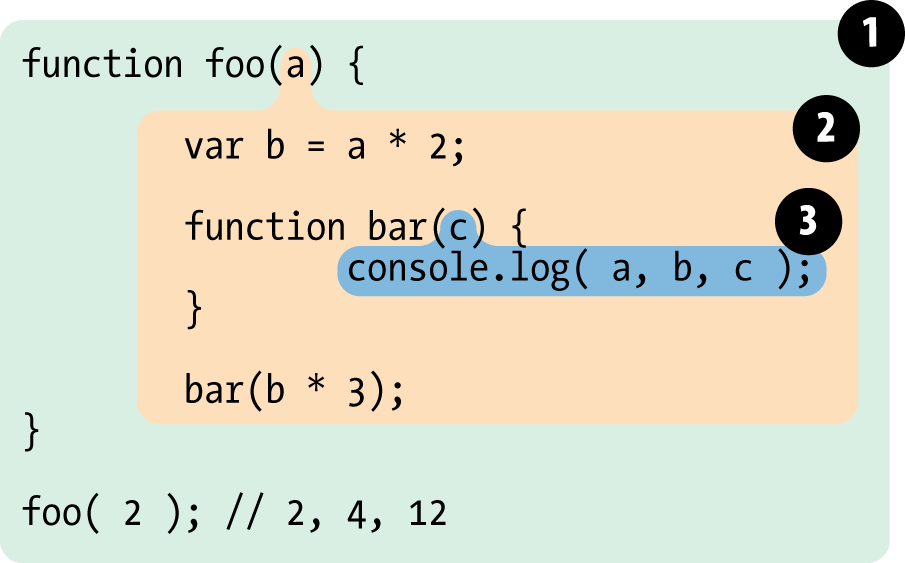
\includegraphics{fig2.png}
\caption{Scope as bubbles \cite{getify}}
\end{figure}

\section{Survey \& Interviews}\label{survey-interviews}

To form a general understanding of how IDEs and some of their specific
features are used, an online survey targeted towards professional
developers was created. The survey ran in April 2014 over the course of
two weeks and yielded answers from 45 participants.

Besides general questions, e.g. which programming languages and IDEs the
participants used, it collected information about the usage of the
following IDE functionalities:

\begin{itemize}
\itemsep1pt\parskip0pt\parsep0pt
\item
  Navigation of code
\item
  Debugging
\item
  Usage of API and language documentation
\item
  Autocompletion
\item
  Project structure and scaffolding
\item
  Asynchronicity
\item
  Syntax Highlighting
\end{itemize}

For each of the areas it was asked if and how the participants were
using them and—if appropriate—how their IDE was supporting them. They
survey instrumented multiple-choice questions with an additional „Other“
field for custom answers, as well as open-ended questions with a
free-form text field.
